\section{The Disaster Scenario}
\label{sec:scenario}

\noindent We consider a disaster scenario involving a satellite, powered radioactive fuel, that has crashed in a sub-urban area (see Section \ref{atomic} to see how this helps implement a  mixed-reality game). While debris is strewn around a large area, damaging buildings and causing accidents and injuring civilians, radioactive particles discharged in the air, from the debris, are gradually spreading over the area, threatening to contaminate food reserves and people. Hence, emergency services, voluntary organisations, and the military are deployed to help evacuate the casualties and resources before these are engulfed by a radioactive cloud.  In what follows, we model this scenario formally and then describe the optimisation problem faced by the actors  (i.e., including emergency services, volunteers, medics, and soldiers) in trying to save as many lives and resources as possible.  We then propose an algorithm to solve this optimisation problem (in Section \ref{sec:algo}). In Section \ref{sec:atomic}, we demonstrate how this algorithm can be used by a software agent (in our mixed-reality game) in a mixed-initiative process to coordinate field responders. 

\subsection{Formal Model}
\noindent Let $G$ denote a grid overlaid on top of the disaster space, and the satellite and actors are located at various coordinates $(x,y) \in G$ in this grid. The radioactive cloud induces a radioactivity level  $l \in [0,100]$ at every point it covers in the grid (100 corresponds to maximum radiation). While the exact radiation levels can be measured by responders on the ground (at every grid coordinate) using their geiger counter, it is assumed that some information is available  from existing sensors  in the area. However, this information is uncertain due to the poor positioning of the sensors and the variations in wind speed and direction (and we show how this uncertainty is captured in the next section). A number of safe zones $G' \subseteq G$ are defined where the responders can drop off assets and casualties. Let the set of $n$ field responders be denoted as $p_1, \cdots p_i \cdots, p_n \in I$ and the set of $m$s rescue tasks as  $t_1,\cdots, t_j, \cdots, t_m\in T$.  As responders enact tasks, they may become tired, get injured, or receive radiation doses that may, at worst, be life threatening. Hence, we assign each responder  a health level $h_i\in [0,100]$ that decreases based on their radiation dose (\textbf{Wenchao: what's the relationship between radiation dose and health decrease?}) and assume that their decision to perform the task allocated to them is liable to some uncertainty (e.g., they may not want to do a task because they are tired or don't believe it is the right one to do). Moreover, each responder has  a specific role  $r \in Roles$ (e.g., fire brigade, soldier, or medic) and this will determine the capabilities he or she has and therefore the tasks he or she can perform. We denote as $Roles(p_i)$ the role of responder $p_i$. In turn, to complete a given task $t_j$,  a set of responders $I' \subseteq I$ with specific roles $R_{t_j} \subseteq R$ is required. Thus, a task can only be completed by a team of responders $I'$ if $\{Roles(p_i) | p_i \in I'\} = R_{t_j}$. 
\begin{figure}[htbp]
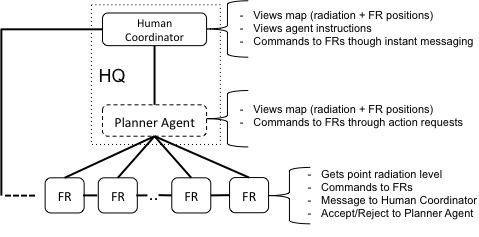
\includegraphics[width=\columnwidth]{scenario.jpg}
\label{fig:scenario}
\caption{The interactions between different actors in the disaster scenario. Lines represent communication links. Planner agent and coordinator sit in the headquarters (HQ). Field responders (FRs) can communicate with all actors directly.}
\end{figure}
In our scenario, we assume that the field responders are coordinated by the headquarters headed by a human coordinator $H$ but assisted by a planner agent $PA$ that can receive input from the human coordinator or the field responders.  While the human coordinator $H$ communicates its instructions directly to the responders (e.g., using an instant messaging client or walkie talkie), the planning agent $PA$ can compute an allocation of tasks for the responders to complete. This is communicated to them in terms of simple "Do task X at position Y". The responders may not want to do some tasks (for reasons outlined above) and may therefore simply accept or reject the received instruction. These interactions are depicted in Figure \ref{fig:scenario}.  

It is important to note that our model implements different types of control: (i) agent-based: when the agent instructs the responders (ii) human-based: when responders work with the coordinator or between themselves. Our model also captures different modes of control: (i) centralised: when responders respond to the planning agent or human coordinator (ii) decentralised: if responders coordinate between themselves. Crucially, this scenario allows for flexible levels of human and agent autonomy. For example, field responders may simply implement the plan given to them by the planner agent but can also feedback their constraints to the planner agent (as we demonstrate later) by rejecting some instructions and requesting new instructions.

Given this model, we next formulate the optimisation problem faced by the responders  and solved by the planning agent (later  in Section \ref{sec:algo}). To this end, we propose a Multi-Agent Markov Decision Process (MMDP)~\cite{?} that captures the uncertainties of the radioactive cloud and the responders' behaviours. Specifically, we model the spreading of the radiative cloud as a random process over the disaster space and allow the actions requested from the responders to  fail (because they refuse to go to a  task) or incur delays (because they are too slow) during the rescue process. This stands in contrast to previous work \cite{csftp,HTSSC} that require the process of task executions to be deterministic and explicitly model the task deadlines as deterministic constraints (which are stochastic in our domain). Thus in the MMDP model, we represent  task executions as stochastic processes of state transitions. Thus, the uncertainties of the radioactive cloud and the responders' behaviours can be easily captured with transition probabilities. Additionally, modelling the problem as a MMDP allows us to use many sophisticated algorithms such as RTDP and MCTS that have already been well developed in the literature~\cite{?,?,?}.


\subsection{The Optimisation Problem}
\label{sec:model}
\noindent Previous agent-based models for team coordination in disaster response typically assume deterministic task executions and environments \cite{ramchurn:etal:2010,Scerri2005}. However, in order to evaluate agent-guided coordination in a real-world environment, it is important to consider uncertainties due to player behaviours and the environment (as discussed in the previous section). Given this, we propose a new representation for the task allocation problem in disaster response that does take into account such uncertainties. More specifically, we represent this problem using an MMDP that captures the uncertainties of the radioactive cloud and the responders' behaviours. We model the spreading of the radioactive cloud as a random process over the disaster space and allow the actions requested from the responders to  fail (because they decline to go to a  task) or incur delays (because they are too slow) during the rescue process. Thus in the MMDP model, we represent  task executions as stochastic processes of state transitions, while the uncertainties of the radioactive cloud and the responders' behaviours can be easily captured with transition probabilities.  More formally, the MMDP is
represented by tuple $\mathcal{M} = \langle I, S, \{A_i\}, P, R
\rangle$, where $I$ is the set of actors as defined in the previous
section,  $S$ is the state space, $A_i$ is a set of responder
$p_i$'s actions, $P$ is the transition function, and $R$ is the
reward function. We elaborate on each of these below.

In more detail, $S= S^G_r \times S_{p_1} \times \cdots \times
S_{p_n} \times S_{t_1} \times \cdots \times S_{t_m}$ where $S^G_r =
\{l_{(x,y)}| (x, y) \in G\}$ is the state variable of the
radioactive cloud that specifies the radioactive level
$l_{(x,y)}\in[0, 100]$ at every point $(x, y)\in G$. $S_{p_i} =
\langle h_i, (x_i, y_i), t_j \rangle$ is the state variable for
each responder $p_i$ that specifies her health level
$h_i\in[0, 100]$, her present position $(x_i, y_i)$, and the task
$t_j$ she is carrying out. $S_{t_j} = \langle {\tt st_j}, (x_j, y_j)
\rangle$ is then the state variable for task $t_j$ to specify its
status ${\tt st_j}$ (i.e., the target is picked up, dropped off, or idle) and position $(x_j, y_j)$. 

The three types of actions  (in set $A_i$) a responder can take
are: (i) {\em stay} in the current location $(x_i, y_i)$, (ii) {\em
move} to the 8 neighbouring locations, or (iii) {\em complete} a
task located at $(x_i, y_i)$. A joint action $\vec{a}=\langle a_1,
\cdots, a_n \rangle$ is a set of actions where $a_i\in A_i$, one
for each responder (a responder may just \emph{stay} at its current
position if it has no targets to rescue). The transition function
$P$ is defined in more detail as: $P= P_r \times P_{p_1} \times
\cdots \times P_{p_n} \times P_{t_1} \times \cdots \times P_{t_m}$
where:
\begin{itemize}
    \itemsep=-2pt
    \item $P_r(s'_r|s_r)$ is the probability the radioactive
        cloud spreads from state $s_r\in S^G_r$ to $s'_r\in
        S^G_r$. It captures the uncertainty of the  radiation
        levels in the environment due to  noisy sensor readings
        and the variations in wind speed and direction.
    \item $P_{p_i}(s'_{p_i}|s, a_i)$ is the probability
        responder $p_i$ transitions to a new state $s'_{p_i}\in
        S_{p_i}$ when executing action $a_i$. For example, when
        a responder is asked to go to a new location,  she
        may not end up there because  she is tired,
        gets injured, or receives radiation doses that are life
        threatening.
    \item $P_{t_j}(s'_{t_j}|s, \vec{a})$ is the probability
        of task $t_j$ being completed. A task $t_j$ can only be completed by a
        team of responders with the required types ($\Theta_{t_j}$) located at the
        same position as $t_j$.
\end{itemize}

Now,  if  $t_j$ is completed (i.e., in ${\tt st_j}\in S_{t_j}$, the
status ${\tt st_j}$ is marked as ``dropped off'' and its position $(x_j,
y_j)$ is within a safe zone), the team will be rewarded using
function $R$. The team is penalised if a responder $p_i$ gets
injured or receives a high dose of radiation (i.e., in $s_{p_i}$,
the health level $h_i$ is 0). Moreover, we attribute a cost to each
of the responders' actions since  each  action requires them to
exert some effort (e.g., running or carrying objects).


Give the above definitions, a policy for the MMDP is a mapping from
states to joint actions, $\pi: S \rightarrow \vec{A}$ so that the
responders know which actions to take given the current state of
the problem. The quality of a policy $\pi$ is  measured by
its expected value $V^\pi$, which can be computed recursively by
the Bellman equation:
\begin{equation}
  V^\pi(s^\tau) = R(s^\tau, \pi(s^\tau)) + \!\!\!\sum_{s^{\tau+1}\in S}\!\!\!
  P(s^{\tau+1}|s^\tau, \pi(s^t)) V^\pi(s^{\tau+1})
\end{equation}
where $\tau$ denotes the current time point and $\pi(s^\tau)$ is a joint action given $s^\tau$. The goal of solving
the MMDP is to find an optimal policy $\pi^*$ that maximises the
expected value with the initial state $s^0$, $\pi^* =
\arg\max_{\pi} V^\pi(s^0)$.

At each decision step, we assume the planning agent can fully
observe the state of the environment $s$ by collecting sensor
readings of the radioactive cloud and GPS locations of the
responders. Given a policy $\pi$ of the MMDP, a joint action
$\vec{a}=\pi(s)$ can be selected and broadcast to the responders
(as mentioned earlier).

